\chapter{荧光寿命成像}\label{Chap:5}
\section{荧光寿命成像(FLIM)技术概述}\label{5.1}

与传统荧光强度成像主要记录荧光信号的空间分布不同，荧光寿命成像(fluorescence lifetime imaging, FLIM)关注的是荧光分子在受到激发后，从激发态回到基态所经历的平均时间尺度。该时间常数通常位于皮秒至纳秒量级，主要由分子的辐射跃迁与非辐射跃迁共同决定。由于荧光寿命更多反映分子所处微环境及其失活动力学特征，而对探针浓度、激发功率波动、光路不均匀以及组织衰减等因素相对不敏感，因此 FLIM 在复杂生物样品中更适合用于定量分析\cite{RN563}。

在单指数衰减近似下，荧光信号可写为
\begin{equation}
  I(t)=I_0 e^{-t/\tau}
\end{equation}

其中 $I_0$ 为初始荧光强度，$\tau$ 为荧光寿命。此时，$\tau$ 也可理解为荧光强度衰减至初始值 $1/e$ 所对应的时间常数。对于实际生物或化学体系，由于分子微环境往往并不均一，荧光衰减常表现为多指数形式，此时需采用更复杂的衰减模型进行描述\cite{RN2036}。

按实现方式，FLIM 可分为频域法和时域法两大类\cite{RN1623}。其中，时域 FLIM 方法主要包括时间相关单光子计数(time-correlated single photon counting, TCSPC)、脉冲采样(pulse sampling, PS)\cite{RN2118}、时间门控(time gating, TG)\cite{RN2120} 以及条纹相机(streak camera, SC)成像\cite{RN568,RN2075}。在这些方法中，TCSPC 兼具较高时间分辨率和较高灵敏度，被广泛认为是荧光寿命测量的经典方法和技术基础。

随着 Becker \& Hickl GmbH、PicoQuant GmbH 等商业公司的推动，FLIM 已由早期的单点测量逐步发展为可支持多通道、高计数率和活体实时成像的成熟技术平台\cite{RN1656,RN897,RN2050,RN2049}。依托这些硬件基础，FLIM 已被广泛用于温度\cite{RN2037,RN127}、离子浓度\cite{RN2038}、氧浓度\cite{RN2040}、细胞内 pH\cite{RN2042}、蛋白聚集\cite{RN2041} 以及 FRET \cite{RN913,RN1809,RN247} 等生物过程的定量表征。因此，在多光子成像和活体功能成像研究中，FLIM 不仅提供了强度之外的附加维度，也为复杂微环境中的定量分析提供了重要手段。



\subsection{荧光寿命的物理基础}\label{5.1.1}

荧光寿命来源于激发态分子的失活动力学过程。当荧光分子吸收光子后，电子由基态跃迁至激发态；随后，分子可通过多种弛豫途径返回基态。最常见的两类失活过程分别为辐射跃迁(radiative transition)和非辐射跃迁(non-radiative transition)。在辐射跃迁过程中，分子通过发射光子回到基态；而在非辐射跃迁过程中，激发态能量则通过分子振动、热耗散或与周围环境相互作用等方式释放。

分子的吸收、振动弛豫、内部转换以及荧光与磷光发射等过程，通常通过 Jablonski 能级图进行描述。Jablonski 图能够直观展示分子在不同电子态(如 $S_0$、$S_1$、$S_2$)及其振动态之间的跃迁关系。图~\ref{fig4-5}(\subref{fig4})给出了典型的 Jablonski 能级图示意，其中荧光通常来源于第一激发单重态 $S_1$ 的最低振动态向基态 $S_0$ 的辐射跃迁。

\begin{figure}[htbp]
  \centering
  \begin{subfigure}[b]{0.45\textwidth}
    \centering
    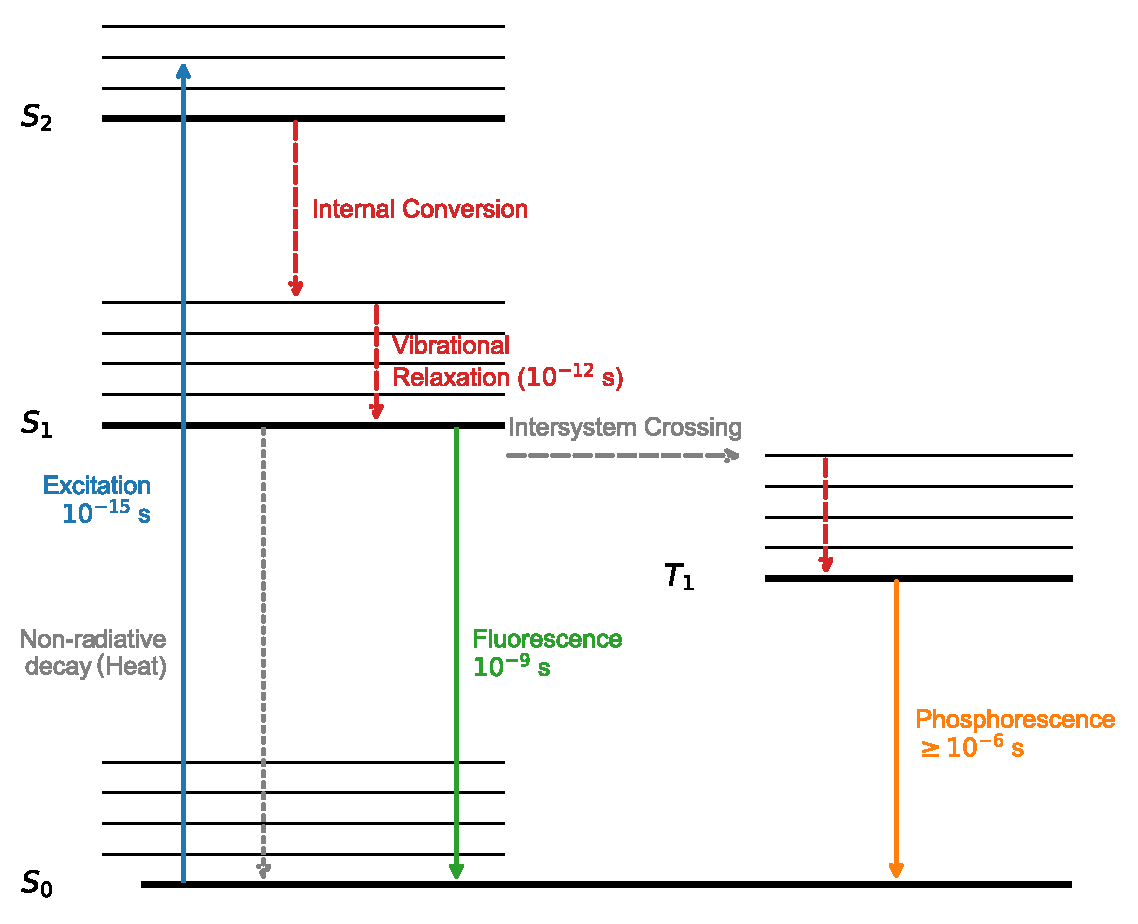
\includegraphics[height = 5cm]{Fig/Fig04.pdf}
    \caption{}
    \label{fig4}
  \end{subfigure}
  \begin{subfigure}[b]{0.45\textwidth}
    \centering
    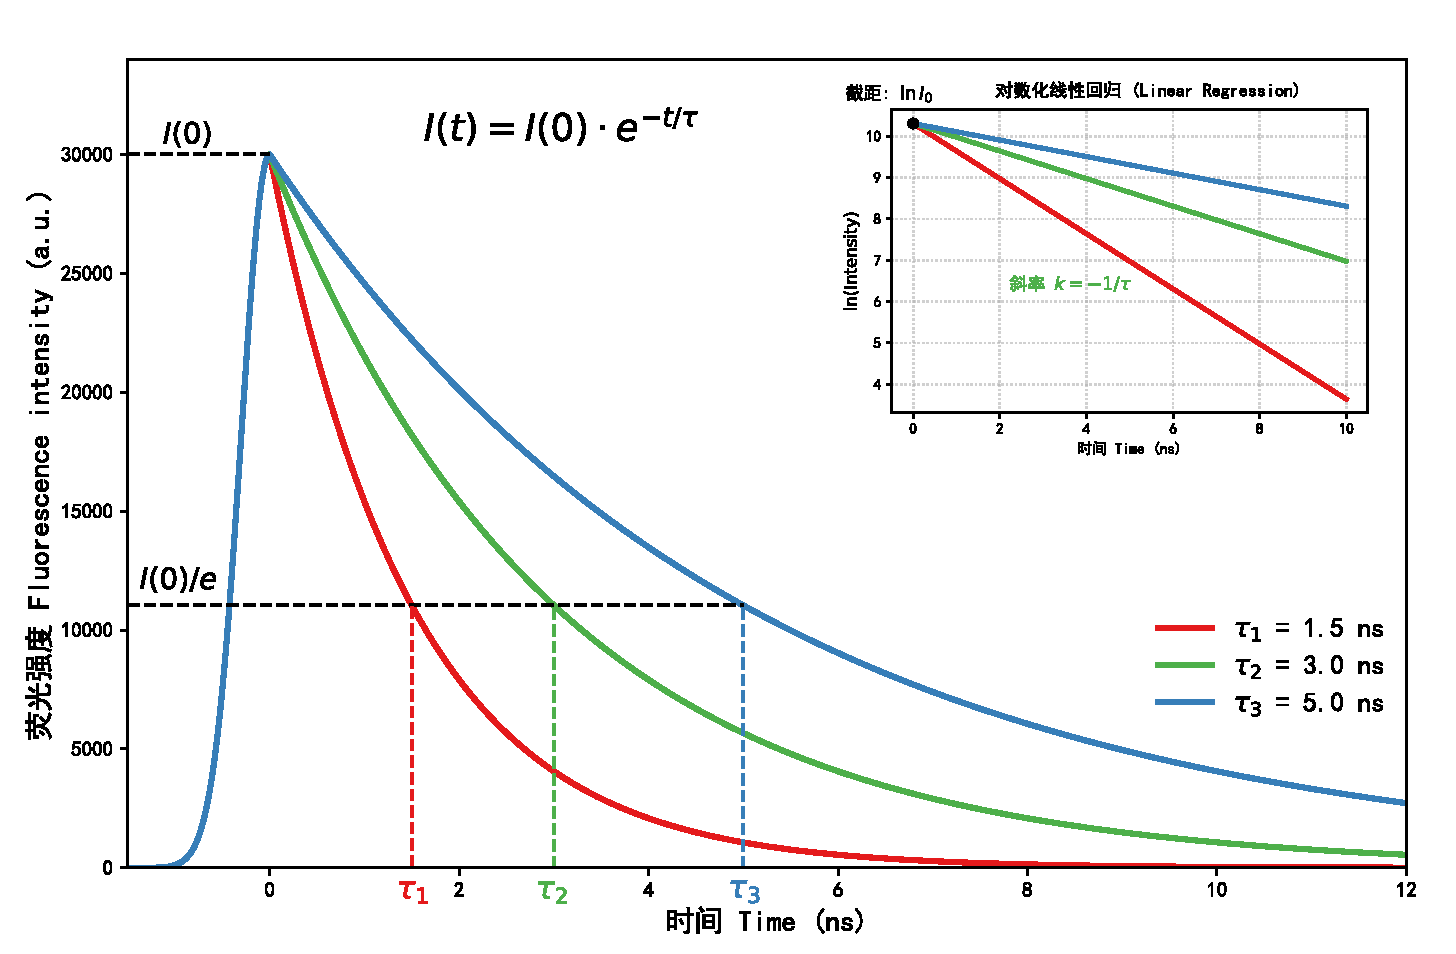
\includegraphics[height = 5cm]{Fig/Fig05.pdf}
    \caption{}
    \label{fig5}
  \end{subfigure}
  \caption{荧光寿命的物理机制与单指数衰减表征示意图。(a) Jablonski 能级图示意；(b) 单指数荧光衰减及其对数线性拟合示意}
  \label{fig4-5}
\end{figure}

》 这里的能级图添加引用或者添加绘图代码

根据 Kasha 定律，无论分子最初被激发到哪个更高激发态，其发光过程通常都发生在最低激发单重态 $S_1$ 的最低振动能级。这是因为分子会在皮秒甚至更短时间尺度内，先通过振动弛豫和内部转换迅速回到 $S_1$ 态的最低振动态，随后再发生荧光发射。因此，大多数荧光发射光谱主要由 $S_1 \rightarrow S_0$ 跃迁决定。

除荧光外，分子还可能通过系间窜越(intersystem crossing, ISC)由单重态跃迁至三重态，例如 $S_1 \rightarrow T_1$。由于三重态到基态的跃迁在量子力学上通常是自旋禁阻的，因此三重态寿命通常远长于单重态，对应的磷光发射时间尺度常可达到微秒至秒量级。对于本文关注的 FLIM 而言，主要测量对象仍然是纳秒量级的荧光衰减过程。

在单指数近似下，若激发态分子的辐射跃迁速率常数和非辐射跃迁速率常数分别为 $k_r$ 和 $k_{nr}$，则激发态总失活速率为两者之和，因此荧光寿命可写为
\begin{equation}
  \tau=\frac{1}{k_r+k_{nr}}
\end{equation}

相应地，荧光量子产率 $\Phi$ 定义为发射荧光光子数与吸收光子数之比，其物理意义是辐射失活在总失活中的占比，因此可表示为
\begin{equation}
  \Phi=\frac{k_r}{k_r+k_{nr}}
\end{equation}

可以看出，寿命 $\tau$ 与量子产率 $\Phi$ 虽然形式相似，但物理含义不同：前者表征激发态持续时间，后者表征辐射发射效率。若定义辐射寿命 $\tau_r=1/k_r$，则还可进一步写为
\begin{equation}
  \Phi = k_r\tau=\frac{\tau}{\tau_r}
\end{equation}

因此，当非辐射过程增强时，寿命和量子产率通常都会下降；反之，当体系更倾向于辐射跃迁时，荧光寿命和量子产率则可能同时提高。



\subsection{荧光衰减模型与寿命提取}\label{5.1.2}

若有 $N(t)$ 个分子处于激发态，则在时间间隔 $dt$ 内，其失活动力学满足
\begin{equation}
  \frac{dN(t)}{dt}=-(k_r+k_{nr})N(t)
\end{equation}

求解该微分方程可得
\begin{equation}
  N(t)=N_0 e^{-t/\tau}
\end{equation}

其中 $\tau=1/(k_r+k_{nr})$。由于荧光发射强度与激发态粒子数成正比，因此单指数衰减模型下的荧光强度可表示为
\begin{equation}
  I(t)=I_0 e^{-t/\tau}
\end{equation}

对于单指数衰减，测得的寿命参数 $\tau$ 与激发态平均寿命在数值上相等。然而，在实际生物样品中，由于荧光分子所处微环境、结合状态或局部淬灭条件往往不均一，荧光衰减常呈现多指数行为，可写为
\begin{equation}
  I(t)=\sum_i A_i e^{-t/\tau_i}
\end{equation}

其中 $\tau_i$ 表示不同衰减组分的寿命，$A_i$ 为对应振幅。对于多指数衰减，常可根据具体应用定义振幅加权平均寿命或强度加权平均寿命，以表征整体衰减过程。

在单指数近似下，对衰减曲线取自然对数可得到
\begin{equation}
  \ln I(t)=\ln I_0-\frac{t}{\tau}
\end{equation}

因此，$\ln I(t)$ 与时间 $t$ 之间呈线性关系，其斜率为 $-1/\tau$，截距为 $\ln I_0$。图~\ref{fig4-5}(\subref{fig5})给出了单指数荧光衰减及其对数线性拟合示意。需要指出的是，这种对数线性回归方法适用于信噪比较高、且衰减行为近似单指数的初步估计；对于实际 TCSPC 数据，通常还需要结合仪器响应函数进行卷积拟合，以获得更准确的寿命结果。

\begin{figure}[htbp]
  \centering
  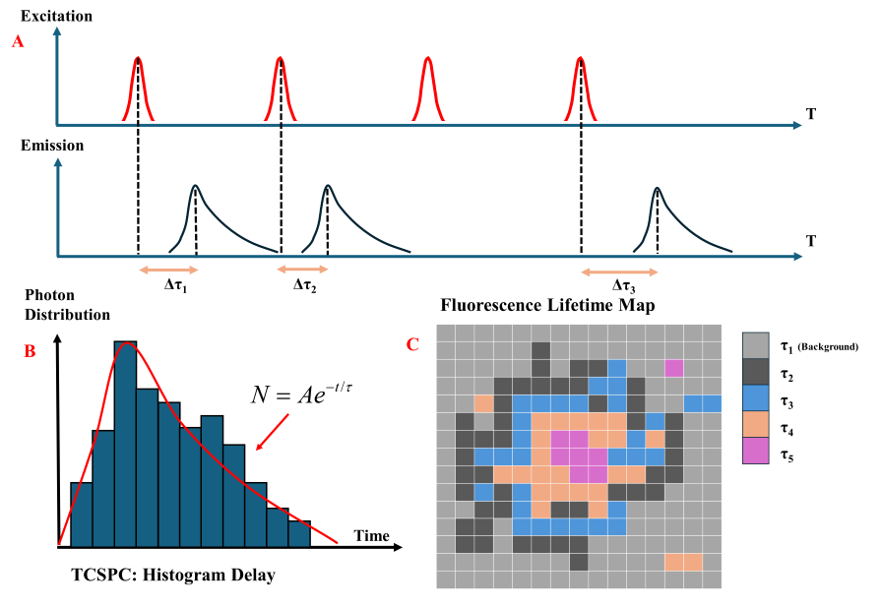
\includegraphics[width=0.8\textwidth]{Fig/Fig06.png}
  \caption{基于 TCSPC 的荧光寿命获取与图像重建示意图}
  \label{fig06}
\end{figure}

图~\ref{fig06} 示意了 FLIM 数据从光子探测到寿命图像重建的基本过程。首先，样品中的荧光分子在脉冲激光激发下吸收光子并产生荧光发射；随后，系统采用 TCSPC 方法对到达探测器的荧光光子进行时间统计，并在每个像素位置建立对应的荧光衰减直方图。通过对该衰减曲线进行寿命拟合，可获得该像素对应的寿命参数 $\tau$。最终，将逐像素拟合得到的寿命值重新映射到空间坐标中，即可形成荧光寿命图像。图中不同颜色代表不同的荧光寿命，从而反映样品内部不同微环境或不同分子状态的空间分布。




\section{仪器响应函数(IRF)标定与同步延迟校准}\label{5.2}

在 FLIM 系统中，仪器响应函数(instrument response function, IRF)用于表征探测链路与 TCSPC 计时电子学共同引入的时间展宽，是寿命拟合与反卷积分析的基础参数。理想情况下，若输入信号为近似瞬时脉冲，则系统输出的时间响应即为 IRF。实际实验中，通常采用尿素晶体等样品产生的二次谐波(second harmonic generation, SHG)信号作为近似瞬时响应，以测定系统 IRF。

除 IRF 标定外，还需校准同步参考信号与荧光探测信号之间的相对时序\cite{RN94}。由于电信号在电缆中的传播速度低于真空光速，因此不同长度的同轴电缆会引入固定的传播延迟，其延迟可表示为
\begin{equation}
  t_d=\frac{L}{v}=\frac{L}{VF\cdot c}
\end{equation}

其中 $L$ 为电缆长度，$v$ 为电信号在电缆中的相速度，$VF$ 为速度因子(velocity factor)，$c$ 为真空光速。对于常见聚乙烯介质同轴电缆，通常有 $VF\approx 0.66$，因此传播延迟近似为

\begin{equation}
  t_d \approx 5.0~\text{ns/m}\;(\approx 1.5~\text{ns/ft})
\end{equation}

若电缆长度变化为 $\Delta L$，则其引入的时间偏移满足
\begin{equation}
  \Delta t \approx \frac{\Delta L}{VF\cdot c}\approx 5.0~\text{ps/mm}\cdot \Delta L
\end{equation}

该延迟会改变荧光衰减曲线在 TCSPC 时间采样窗口中的位置，从而影响寿命拟合的稳定性与准确性。因此，需要结合标准寿命样品对同步时序进行校准，通过调整同步电缆长度，或等效地修改 TCSPC 的时间零点与同步偏置参数，使衰减曲线落在合适的采样窗口内，并获得与标准值一致的拟合寿命。

从系统实现角度看，IRF 标定与同步延迟校准分别对应两类不同问题：前者解决的是``系统本身会将一个理想瞬时信号展宽到什么程度''，后者解决的是``参考时钟与探测信号在时间轴上是否正确对齐''。只有同时完成这两类校准，后续寿命拟合结果才具有可比性和可靠性。

% 如果你后面有 IRF / 时序图，可以加在这里
% \begin{figure}[htbp]
%   \centering
%   \includegraphics[width=0.75\textwidth]{Fig/XXX.pdf}
%   \caption{IRF 测量与同步延迟校准示意图。}
%   \label{fig:irf_sync}
% \end{figure}




\section{FLIM 数据采集与同步模式设计}\label{5.3}

在点扫描 FLIM 系统中，寿命信息的获取不仅依赖于探测器和 TCSPC 电子学本身，还依赖于扫描时序与采集时序之间的严格对应关系。与宽场相机直接输出二维图像不同，点扫描系统中的每一个像素都对应一段时间窗内的光子统计结果，因此必须通过同步信号将``光子到达时间''与``当前扫描位置''正确关联，才能最终重建出荧光寿命图像。也正因为如此，数据采集方式和同步模式的设计，直接决定了 FLIM 图像重建的效率、精度与适用场景。



\subsection{点扫描系统中的时序同步关系}\label{5.3.1}

在点扫描显微镜中，图像采集通常遵循像素(pixel)、行(line)和帧(frame)三级扫描时序。对于一幅 $N\times M$ 像素的扫描图像，系统在完成一个像素的积分后，依次切换至下一像素；当一行中的 $N$ 个像素全部扫描完毕后，产生一次行同步信号(line sync)；当全部 $M$ 行扫描结束后，则产生一次帧同步信号(frame sync)。因此，像素同步信号、行同步信号和帧同步信号共同构成了点扫描 FLIM 图像重建的基本时序框架。

\begin{figure}[htbp]
  \centering
  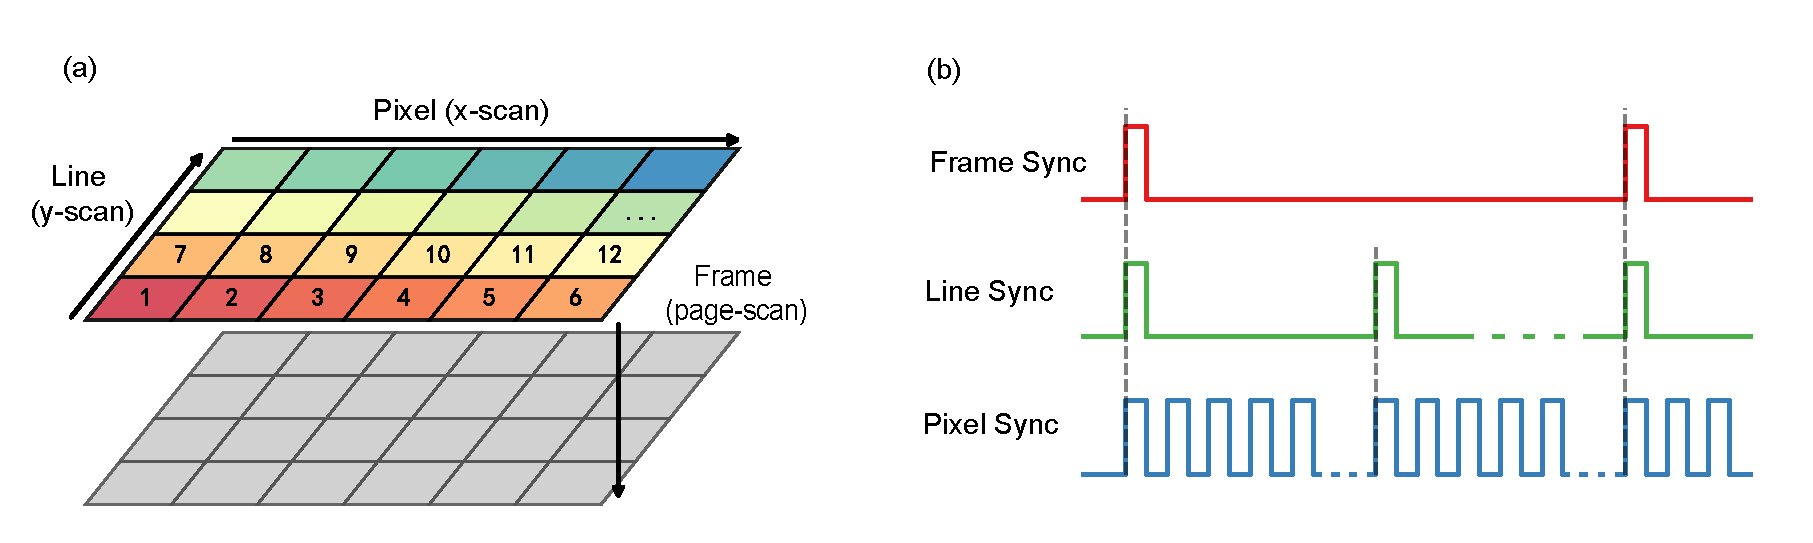
\includegraphics[width=0.8\textwidth]{Fig/Fig18.pdf}
  \caption{点扫描图像重建与多级同步信号之间的时序关系示意图}
  \label{fig18}
\end{figure}

图~\ref{fig18} 给出了点扫描显微镜中的图像重建过程及其对应的多级同步信号关系。图中上部表示像素、行和帧三个层级的扫描顺序；下部则示意了相应的 pixel sync、line sync 和 frame sync 信号。可以看出，图像重建并不是简单地记录光子事件，而是要在多级同步信号约束下，将时间信息重新映射到对应的空间位置中。

在此基础上，本文采用了两类不同的 FLIM 数据采集模式：一类是单路同步采集模式，另一类是三路同步采集模式。两种方式各有特点，分别适用于不同的成像任务与硬件条件。




\subsection{单路同步采集模式}\label{5.3.2}

单路同步模式可视为一种逐像素寿命获取策略。在该模式下，系统仅使用一路触发信号控制寿命数据的采集与保存，即当触发信号到来时，采集卡开始对当前扫描位置对应的荧光时间信息进行记录。每个像素点的寿命数据被单独保存，随后再结合扫描顺序或像素坐标信息，将这些独立数据重新映射为完整的二维寿命图像。

这种方式的优点在于控制结构相对简单，易于在自研硬件和非标准扫描流程下实现，并且对不规则扫描区域或自定义 ROI 成像具有较高灵活性。对于需要逐点分析、逐点存储或特殊扫描路径控制的实验任务，单路同步模式具有较强适配性。

然而，单路同步模式也存在明显不足。由于系统需要为每个像素单独完成数据记录与保存，整体采集效率较低。当扫描视场扩大或像素数增加时，总采集时间会迅速增长；同时，生成的数据文件数量也会显著增加，不仅占用较大存储空间，还会加重后续图像重建与数据管理负担。因此，这种方式更适合中小规模数据采集、方法验证和灵活扫描，而不利于高速、大视场或高通量 FLIM 成像。

\begin{figure}[htbp]
  \centering
  \begin{subfigure}[b]{0.42\textwidth}
    \centering
    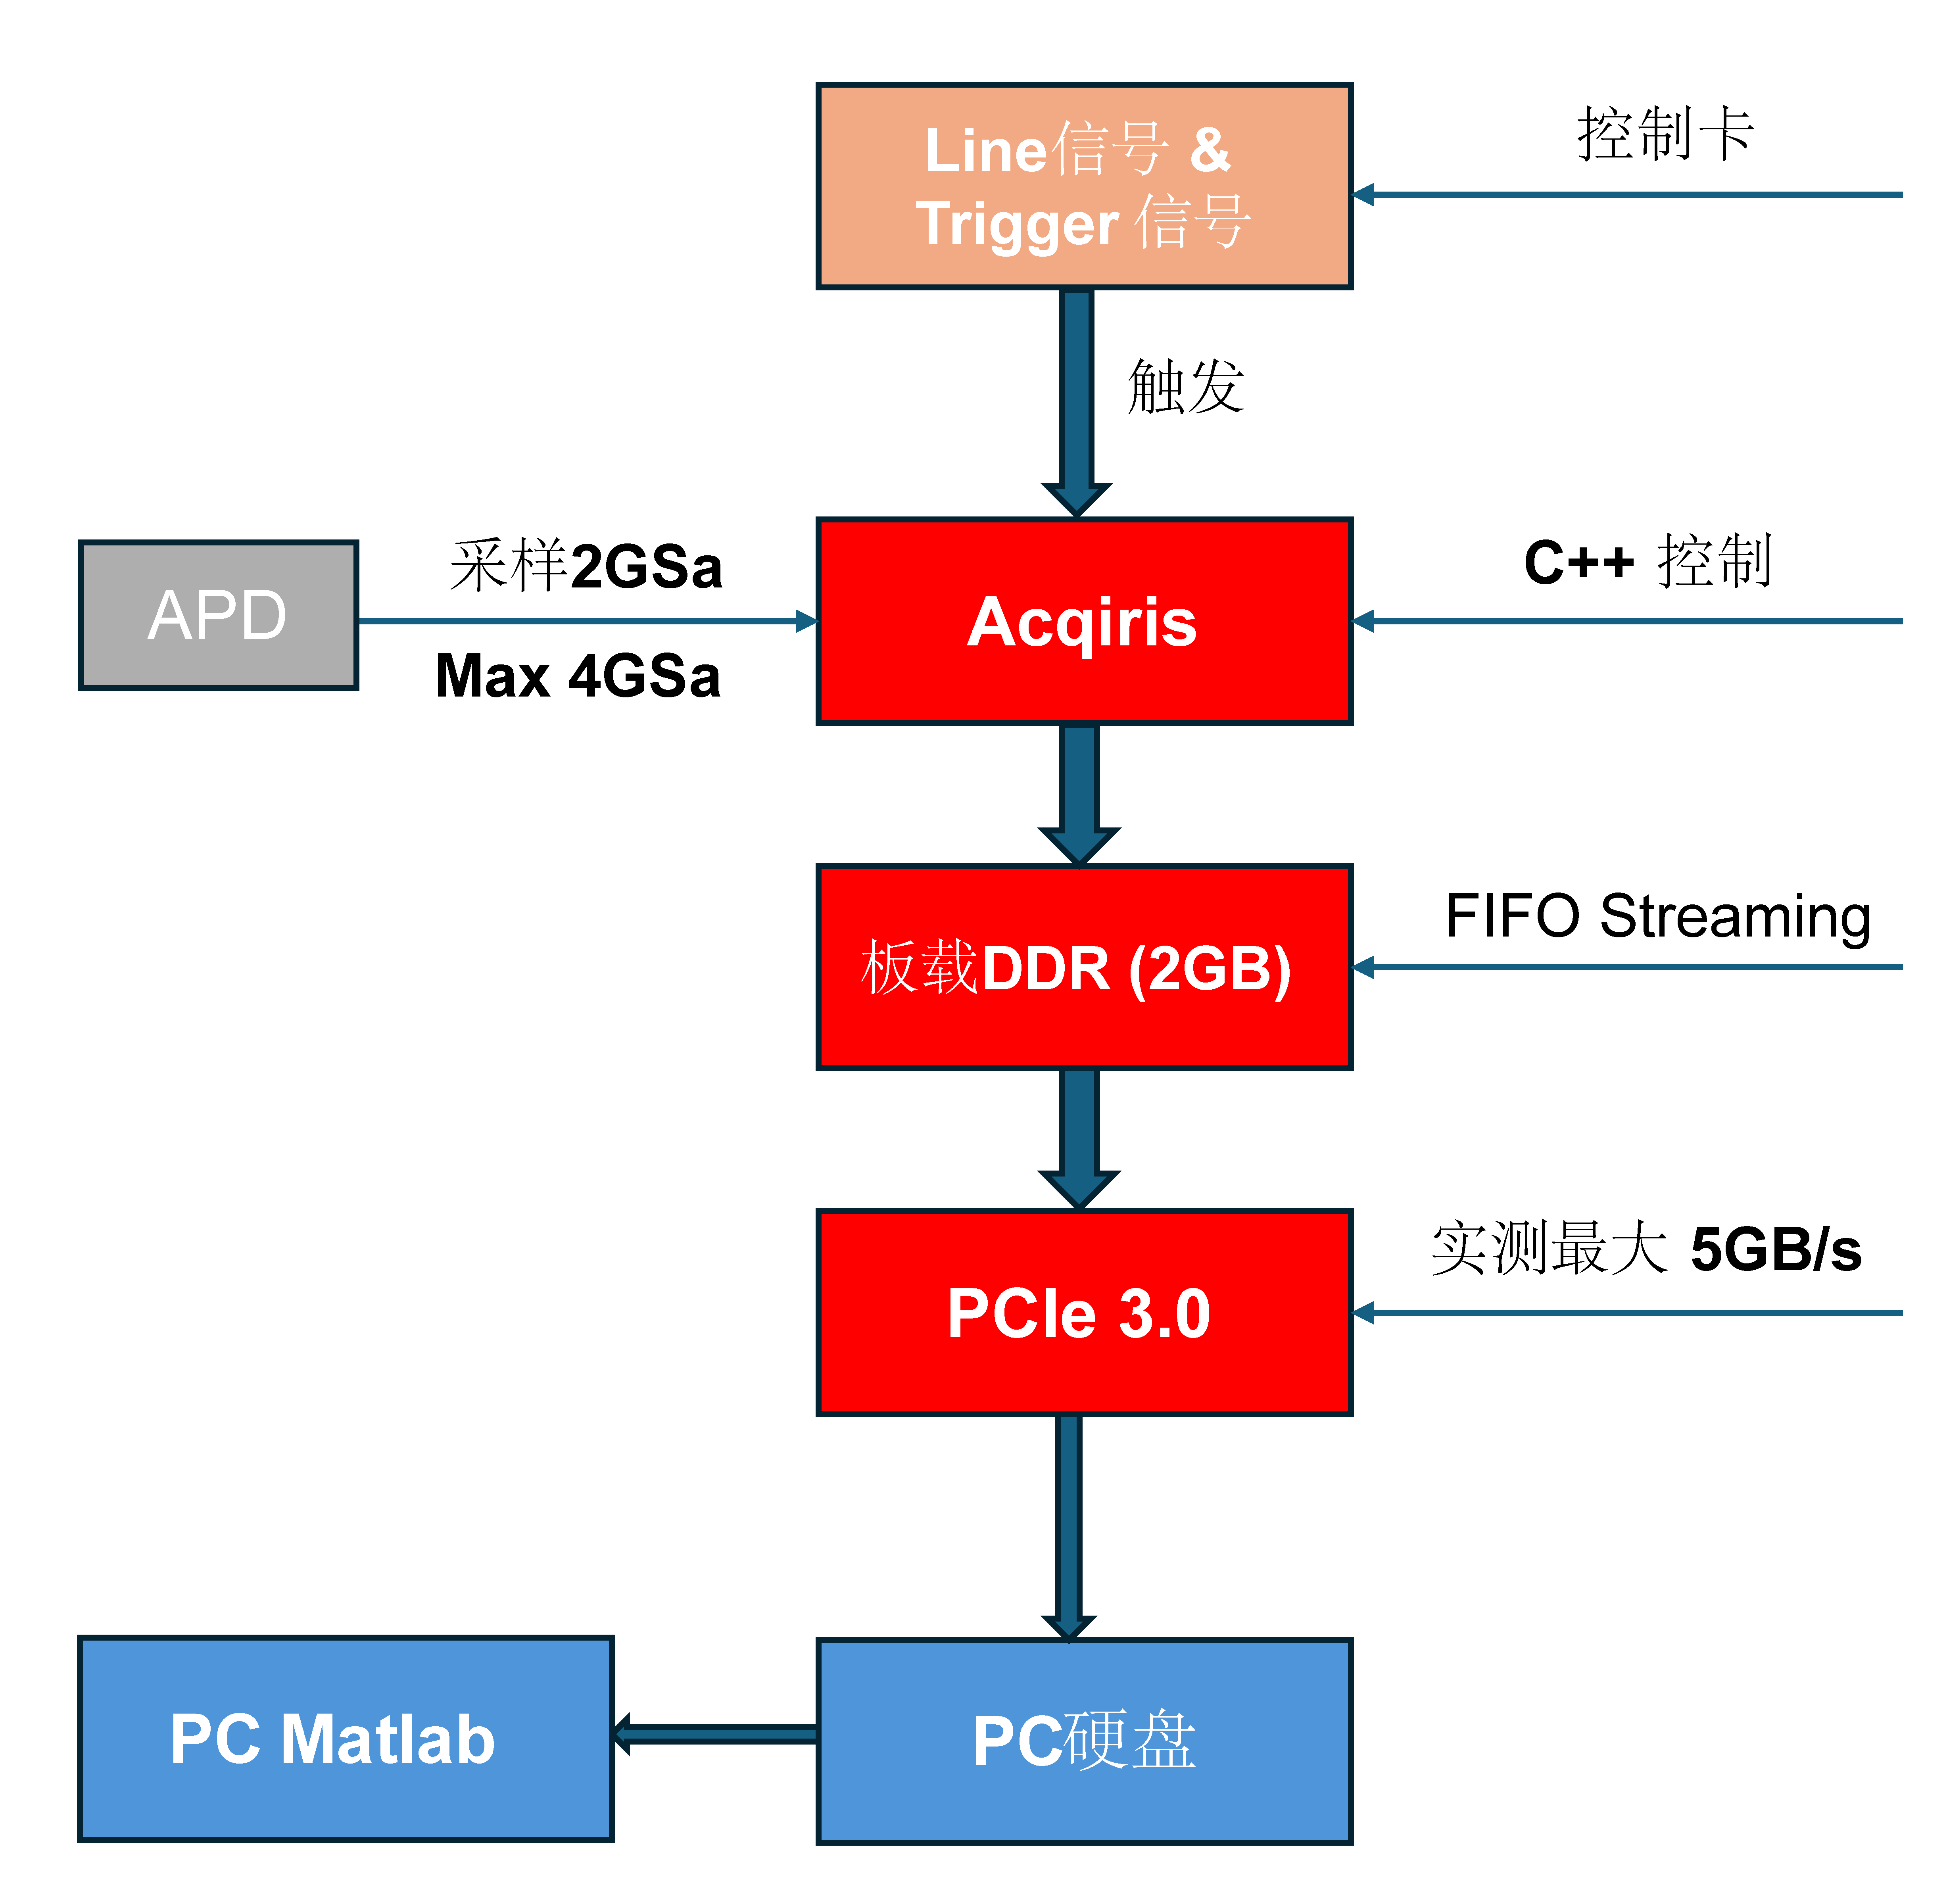
\includegraphics[width = \textwidth]{Fig/Fig19.pdf}
    \caption{}
    \label{fig19}
  \end{subfigure}
  \hfill
  \begin{subfigure}[b]{0.56\textwidth}
    \centering
    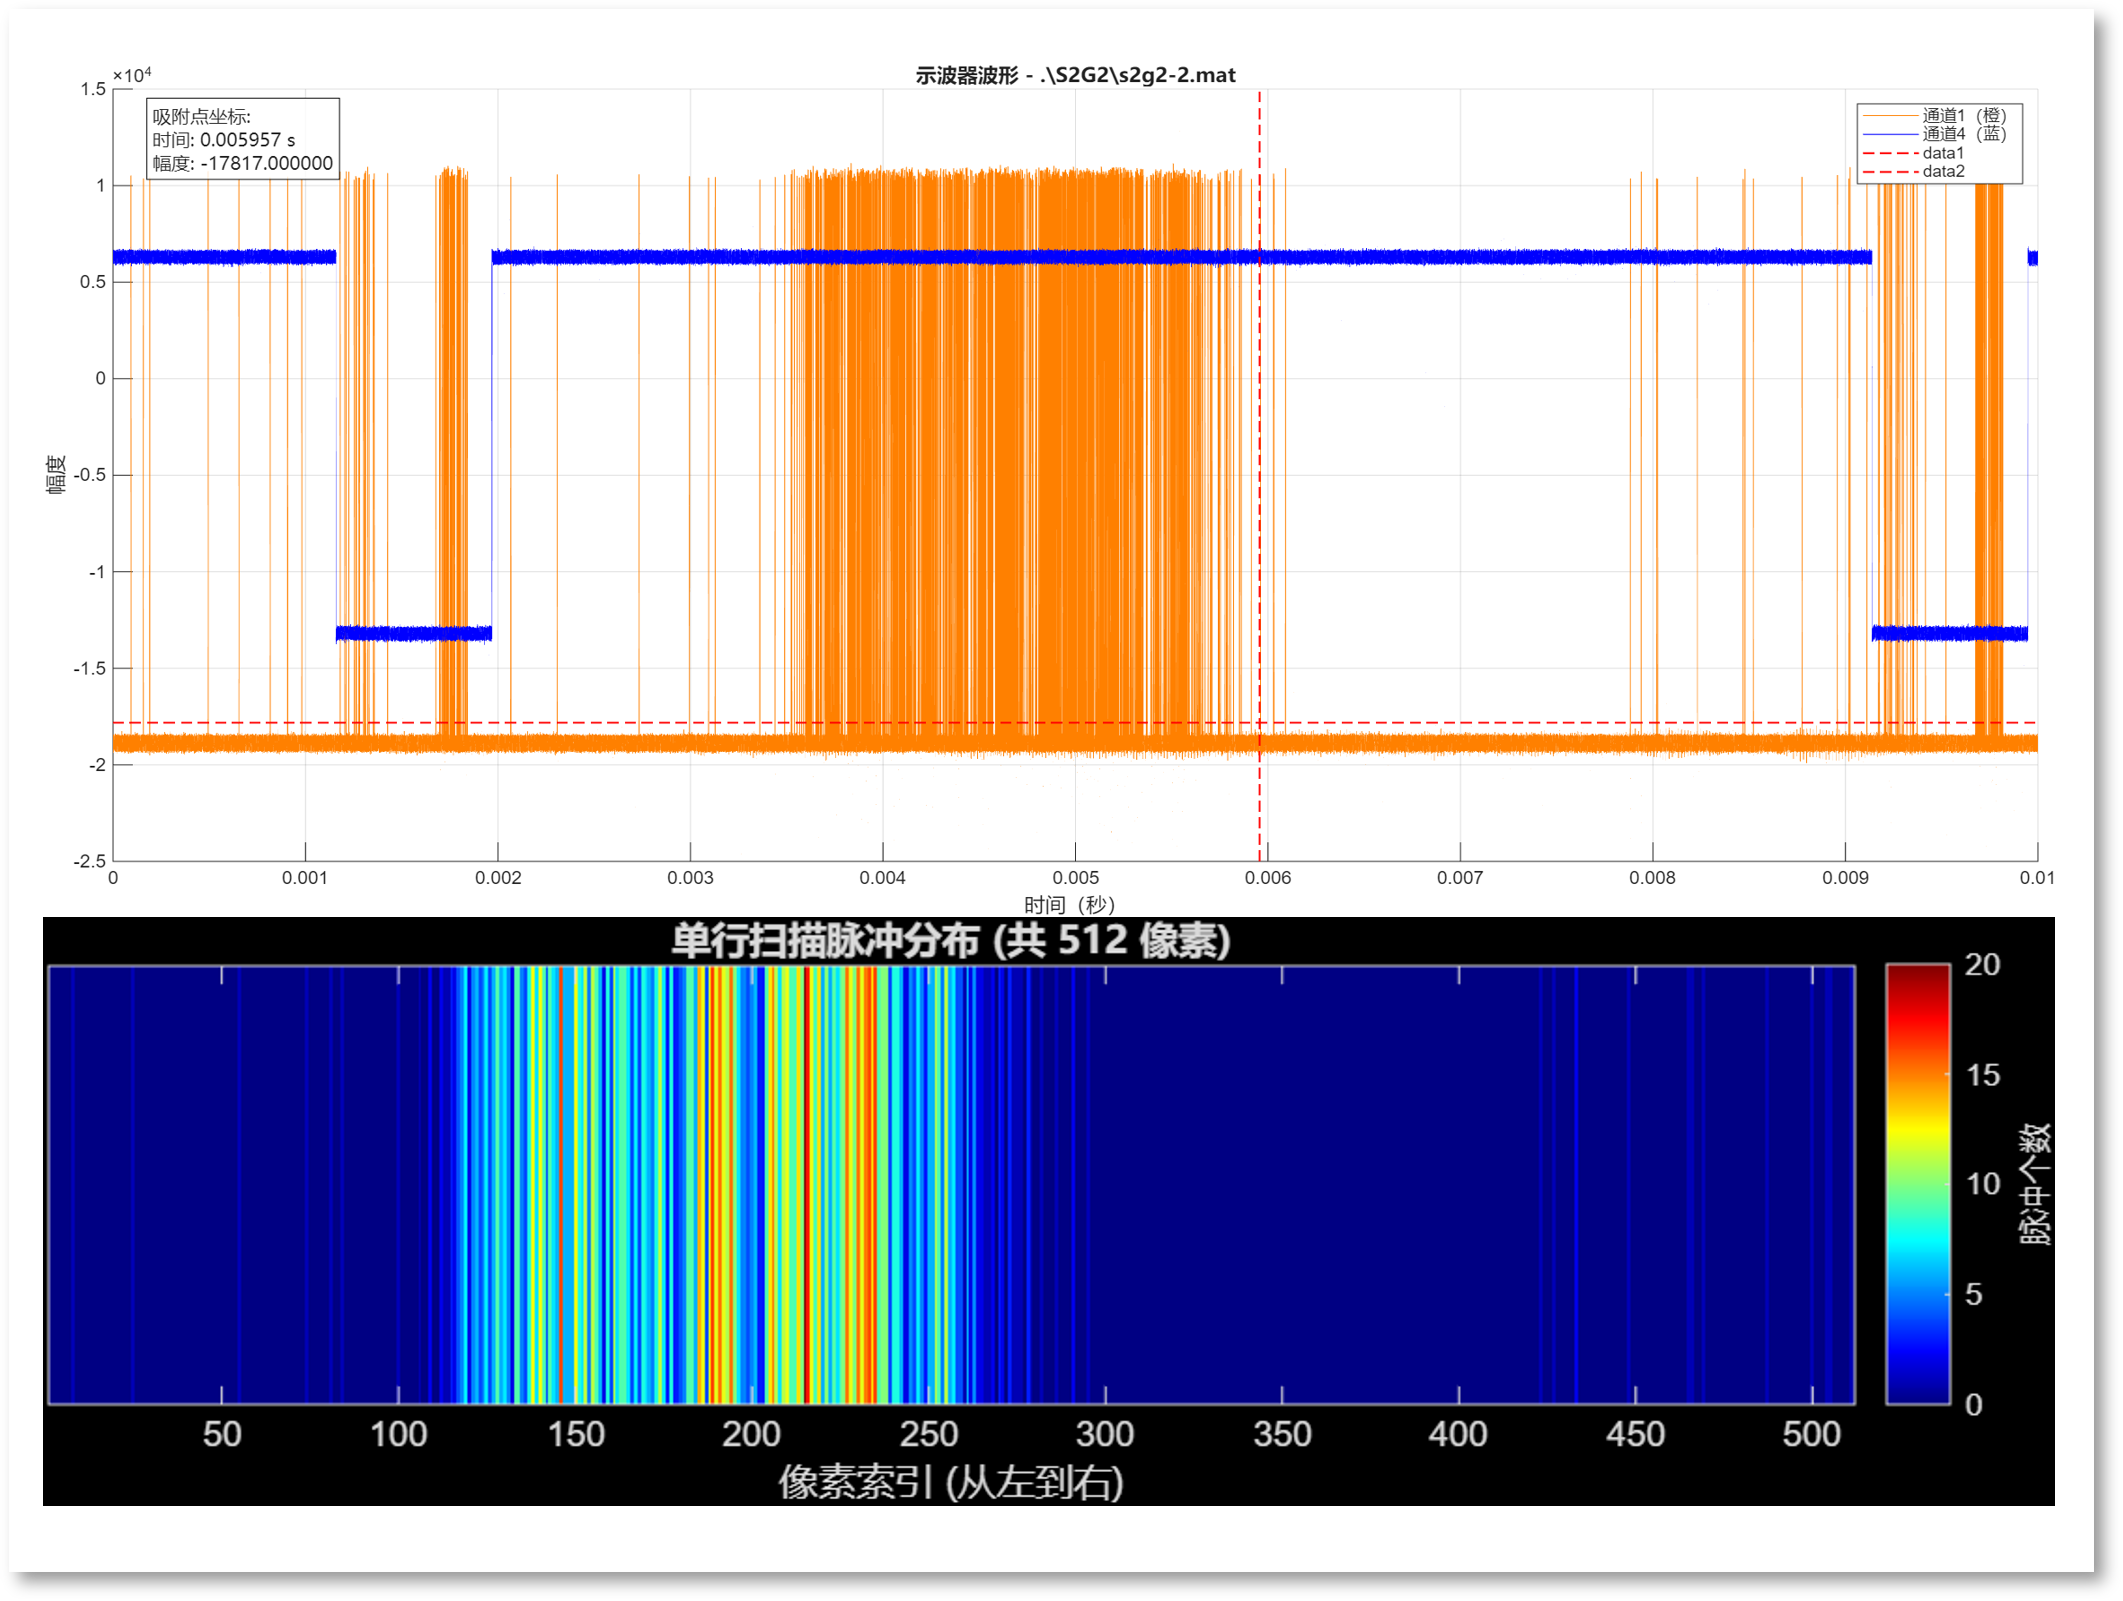
\includegraphics[width = \textwidth]{Fig/Fig20.png}
    \caption{}
    \label{fig20}
  \end{subfigure}
  \caption{单路同步采集模式中的数据流与采样分布示意。(a) 单路同步模式下的数据采集流程；(b) 单路同步下某一行信号的光子分布密度}
  \label{fig19-20}
\end{figure}

图~\ref{fig19-20}(\subref{fig19})展示了单路同步模式下的数据采集流程。除 CPU 端部分处理可并行执行外，数据触发、读取、保存与重分配等关键环节大多需要顺序进行，因此系统总体采集带宽通常受限于链路中最慢的环节，表现出典型的``木桶效应''。这意味着单路同步模式虽然实现简单，但在高数据量场景下容易受到存储与数据吞吐带宽的限制。

图~\ref{fig19-20}(\subref{fig20}) 则给出了单路同步模式下一行扫描数据的示波器观测结果及其数字化重分配示意。蓝色通道表示 line 信号的起止，橙色信号表示对应荧光响应；下方则示意将该行数据重分配到 512 个像素后的信号密度分布。可以看出，不同像素位置的光子密度并不均匀，在高信号区域可能出现局部采样密集，而在低信号区域则可能存在欠采样风险。因此，在单路同步模式下，采样率、扫描速度与像素数之间的匹配关系是系统设计中必须考虑的重要问题。



\subsection{三路同步采集模式}\label{5.3.3}

\begin{figure}[htbp]
  \centering
  \begin{subfigure}[b]{0.7\textwidth}
    \centering
    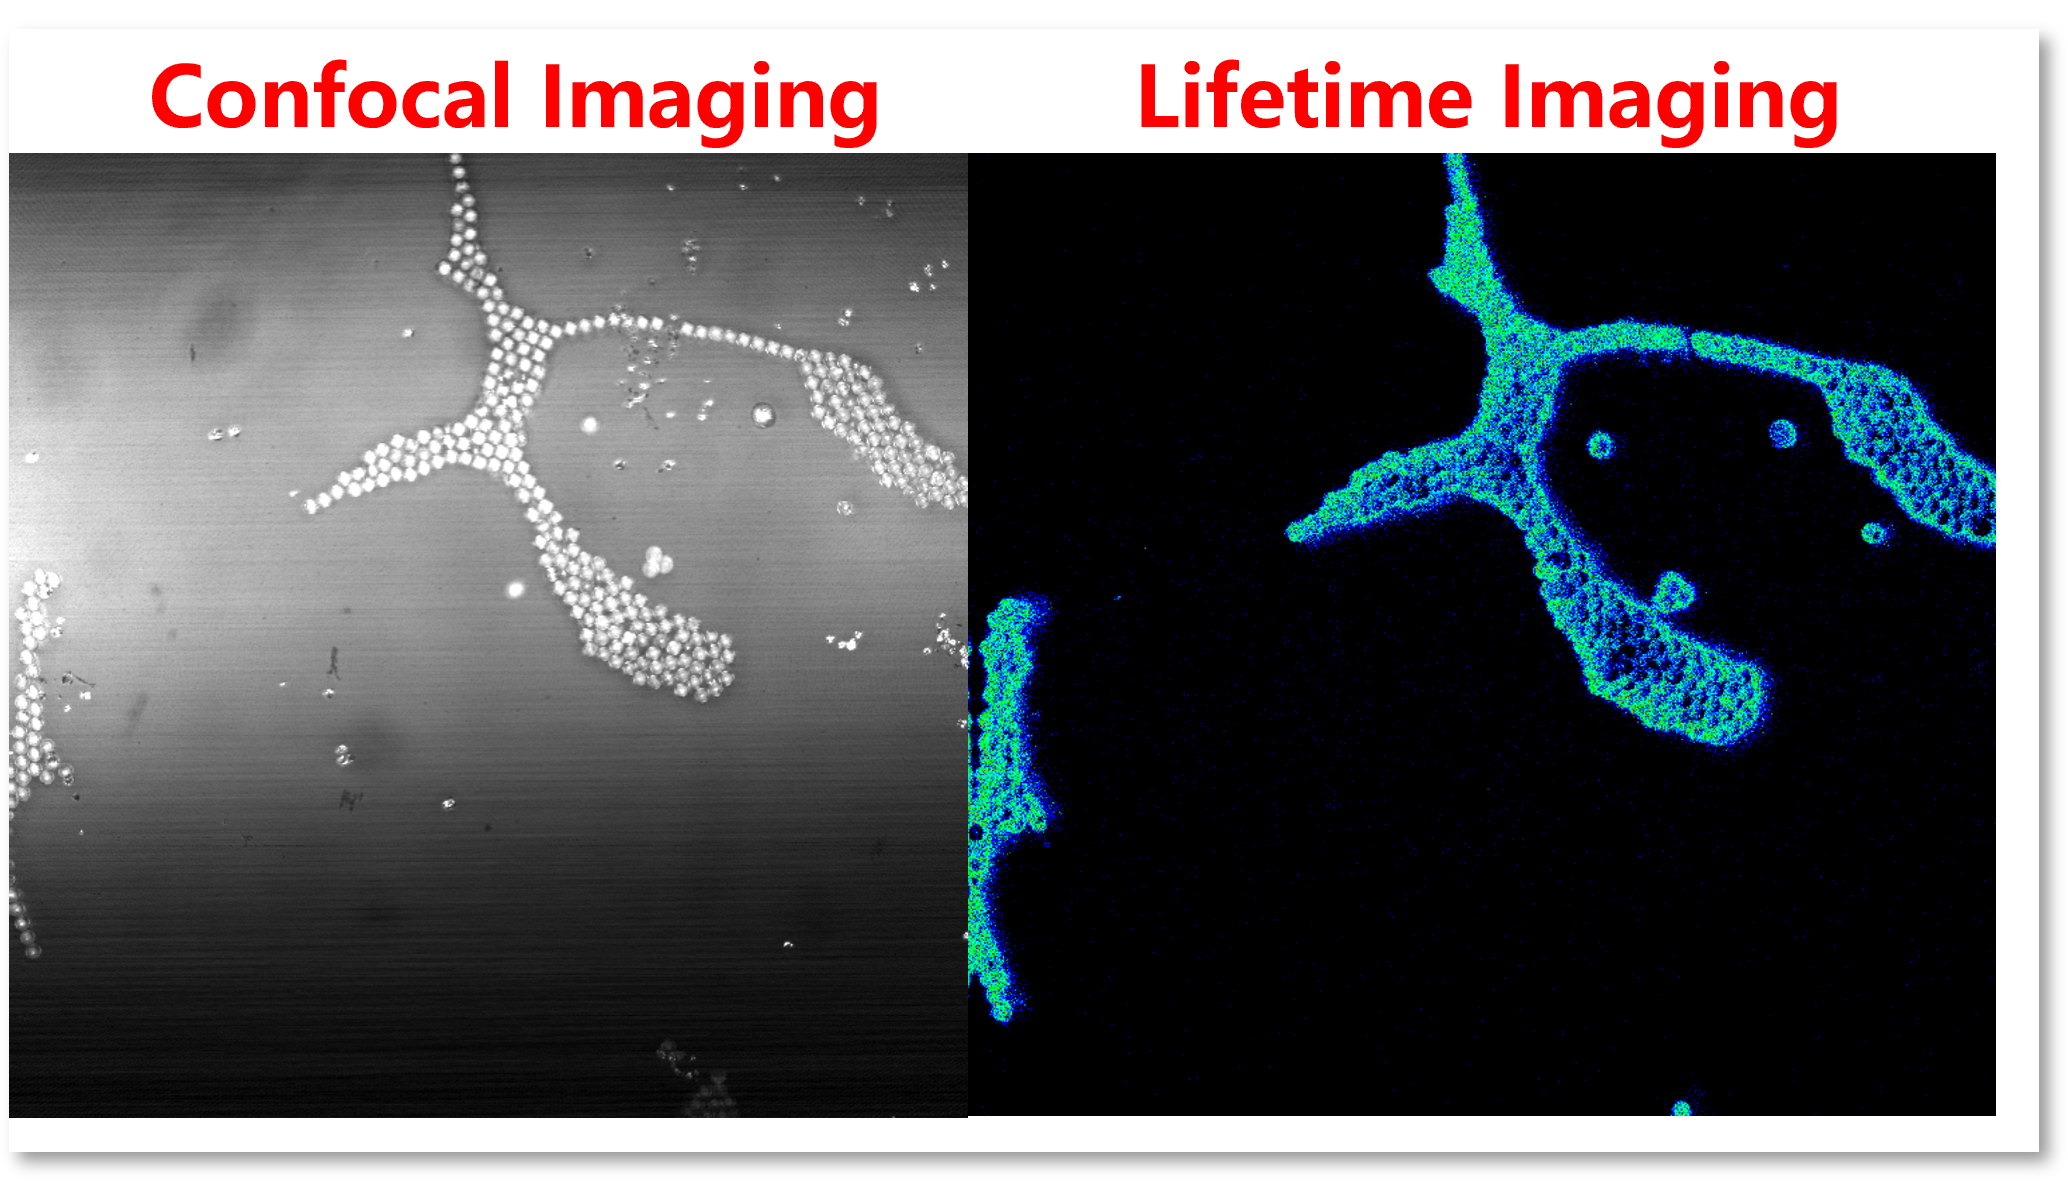
\includegraphics[width=\textwidth]{Fig/Fig21.png}
    \caption{}
    \label{fig21}
  \end{subfigure}

  \vspace{0.2cm}

  \begin{subfigure}[b]{0.7\textwidth}
    \centering
    \includegraphics[width=\textwidth]{Fig/Fig22.png}
    \caption{}
    \label{fig22}
  \end{subfigure}
  \caption{三路同步模式下的荧光寿命成像结果及其与反射式图像、激发功率之间的关系。(a) 反射式共聚焦图像与三路同步 FLIM 图像对比；(b) 不同激发功率条件下的 TCSPC 成像结果}
  \label{fig21-22}
\end{figure}


与单路同步不同，三路同步模式同时引入像素、行和帧三类同步信号，用于协调寿命信息的采集、缓存与写入过程。该模式通常依赖 TCSPC 板卡内部的 FIFO 缓冲与图像文件预分配机制：系统首先预先建立与扫描图像格式对应的寿命图像文件，随后 TCSPC 记录到的光子数据在 pixel、line 和 frame 三类同步信号的共同控制下，按照既定顺序直接写入相应像素位置，从而实现扫描过程与寿命图像生成过程的同步进行。

相较于单路同步模式，三路同步模式的最大优点在于成像效率更高。由于系统能够直接利用多级同步信号完成寿命数据与扫描坐标的对应关系建立，因此在规则矩形区域的栅格扫描中，可直接生成寿命图像，而无需在后处理阶段再进行复杂的逐像素重构。这使得三路同步模式特别适用于标准扫描视场下的快速 FLIM 成像。

但与此同时，三路同步模式对扫描方式的规则性要求更高。当成像区域不是标准矩形，或者各扫描行对应的像素数不一致时，数据组织和图像重建会变得更加复杂，从而降低该模式对不规则 ROI 成像的灵活性。因此，三路同步模式更适合规则区域的高速成像，而单路同步模式则更适合灵活路径扫描和特殊实验设计。

图~\ref{fig21-22} 给出了基于三路同步模式获得的 FLIM 图像结果及其与系统功率的关系。图~\ref{fig21-22}(\subref{fig21})，左图为反射式共聚焦成像结果，右图为利用 line、frame 和 sync 三路信号触发 TCSPC 板卡后获得的荧光寿命图像。两者在空间位置上能够良好重叠，说明三路时序同步关系建立正确，系统能够将寿命信息准确映射到对应的扫描位置。

图~\ref{fig21-22}(\subref{fig22}) 下方图像则给出了不同激发功率条件下的 TCSPC 成像结果。可以看出，随着激发功率增加，探测到的荧光信号增强，寿命图像亮度提高；但当功率过高时，系统可能出现局部计数过高、光子堆积和图像过曝等现象，从而影响寿命拟合的准确性。因此，在三路同步模式下，除了保证时序同步成功外，还必须合理控制激发功率与计数率，使系统工作在线性响应和有效计数范围内。



\section{FLIM 系统操作流程与数据处理链路}\label{5.4}

\begin{figure}[htbp]
  \centering
  \begin{subfigure}[b]{0.6\textwidth}
    \centering
    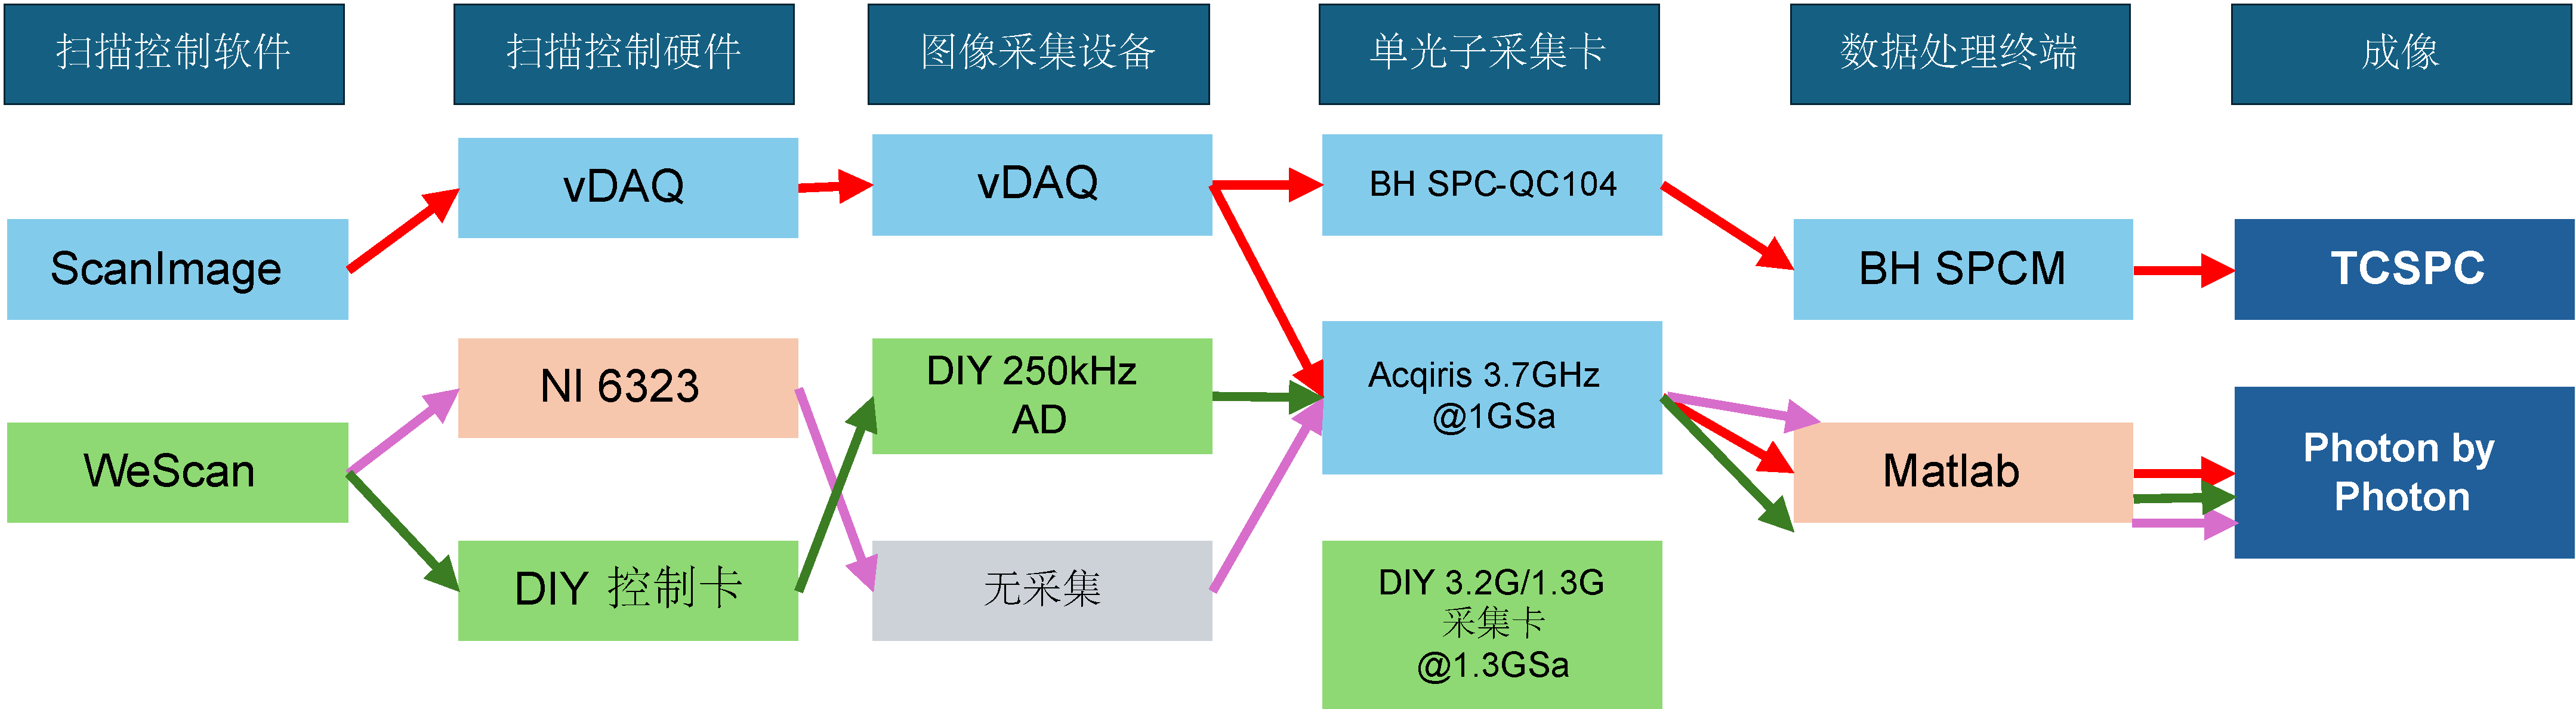
\includegraphics[width=\textwidth]{Fig/Fig24.pdf}
    \caption{}
    \label{fig24}
  \end{subfigure}
  \vspace{0.3cm}
  \begin{subfigure}[b]{0.6\textwidth}
    \centering
    \includegraphics[width=\textwidth]{Fig/Fig24.5.pdf}
    \caption{}
    \label{fig24.5}
  \end{subfigure}
  \caption{FLIM 数据处理链路与多路时序同步关系。(a) 当前已建立的荧光寿命成像处理流程；(b) 三路同步下 Frame、Line、Sync 及其合并信号的时序关系}
  \label{fig24-24.5}
\end{figure}

在完成系统硬件搭建、IRF 标定和同步模式设计后，FLIM 实验还需要依赖明确的数据处理链路，才能将原始光子事件转化为可解释的寿命图像。结合本文所使用的硬件平台与控制方式，目前已建立三类互补的 FLIM 数据处理流程。

如图~\ref{fig24-24.5} 所示，本文目前建立的 FLIM 数据处理流程主要包括以下三类：

第一类为基于商用控制平台的三路同步 FLIM 流程。该流程利用商用 vDAQ 与 ScanImage 软件完成扫描控制与图像采集，并结合商用 TCSPC 板卡实现 pixel、line 和 frame 三路同步寿命成像。其优点是系统成熟、同步关系清晰、能够直接输出规则扫描区域下的寿命图像，适合标准 FLIM 实验和系统性能验证。

第二类为基于自研控制板卡的单路同步 FLIM 流程。该流程中，自研控制板卡的 DA 端口负责输出扫描与运动控制信号，AD 端口负责采集探测器输出，并结合 Acqiris 数据采集卡或自研 3.7\,GHz 采集卡完成单路同步寿命信息记录。该方式更适合灵活扫描、逐点分析和自定义数据处理，也为后续自研高速采集链路提供了平台基础。

第三类为基于单光子计数信号的逐像素重分配与拟合流程。该流程不依赖标准 TCSPC 图像文件的直接生成，而是先通过高速采集卡获取原始光子事件或脉冲响应，再结合扫描坐标信息完成逐像素重分配与寿命拟合。该方式虽然处理流程更复杂，但在硬件选择和算法实现上具有更高自由度，为非标准采集模式和后续算法优化提供了空间。

从实际操作流程看，这三类链路虽然实现方式不同，但基本步骤是一致的：首先完成扫描控制与同步触发，其次获取原始寿命相关数据，再结合同步信号进行空间重建，最后通过寿命拟合得到 FLIM 图像。图~\ref{fig24-24.5}(\subref{fig24.5})给出了三路同步模式下 frame、line、sync信号以及合并触发信号之间的时序关系，说明了寿命采集并不是孤立的计时过程，而是与扫描系统严格耦合的时空映射过程。





\section{FLIM 成像结果与寿命拟合分析}\label{5.5}

在完成系统搭建、同步方式建立以及数据处理流程开发后，本文进一步对荧光寿命成像结果进行了实验验证。图~\ref{fig26} 给出了基于商用 TCSPC 方法和基于单光子计数方法获得的 FLIM 图像结果。

\begin{figure}[htbp]
  \centering
  \begin{subfigure}[b]{0.45\textwidth}
    \includegraphics[width=\textwidth]{Fig/Fig26.png}
    \caption{}
    \label{fig26}
  \end{subfigure}
  \hfill
  \begin{subfigure}[b]{0.49\textwidth}
    \centering
    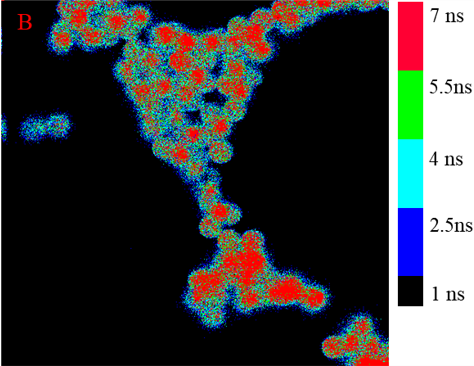
\includegraphics[width=\textwidth]{Fig/Fig27.png}
    \caption{}
    \label{fig27}
  \end{subfigure}
  \caption{反射式、TCSPC、光子计数方式下 FLIM 成像结果。(a) 基于不同采样方式获得的 FLIM 成像结果；(b) 两种不同方式下的荧光寿命对比}
  \label{fig26-27}
\end{figure}

》 这个图注太草率了，需要修改

图~\ref{fig26} 中，子图 A 为使用反射式共聚焦显微镜对 $1\,\mu$m 荧光微球进行成像所得到的参考图像，可作为后续寿命图像空间定位的基准；子图 B 为使用商用 TCSPC 采集卡获得的荧光寿命图像；子图 C 为使用 Acqiris 采集卡在单路同步模式下获得的单光子计数图像，用于后续像素重分配；子图 D 则是在子图 C 完成像素重分配基础上进行逐像素寿命拟合后得到的 FLIM 热力图，其中不同颜色代表不同像素的寿命值。

从结果上看，两种不同方法均能够恢复出样品的寿命分布信息，但初始结果中仍存在由成像功率和系统分辨率设置不当带来的局部过曝与光子堆积问题。为进一步提高寿命拟合质量，本文根据初步结果对成像功率和系统参数进行了优化，并重新采集得到图~\ref{fig27} 所示结果。

图~\ref{fig27}A 为反射式共聚焦图像，用作样品空间分布的参考；图~\ref{fig27}B 为商用 TCSPC 板卡获得的荧光寿命图像，右侧色条表示不同寿命值；图~\ref{fig27}C 表示在单路同步采集条件下，通过优化成像功率和采样参数得到的信号分布；图~\ref{fig27}D 则是在此基础上进行逐像素寿命拟合得到的寿命热图。与优化前相比，优化后的结果能够更清晰地分辨出荧光微球轮廓，并显著减小局部过曝和光子堆积对寿命拟合带来的影响。

\begin{figure}[bhpt]
  \centering
  \begin{subfigure}[b]{0.25\textwidth}
    \centering
    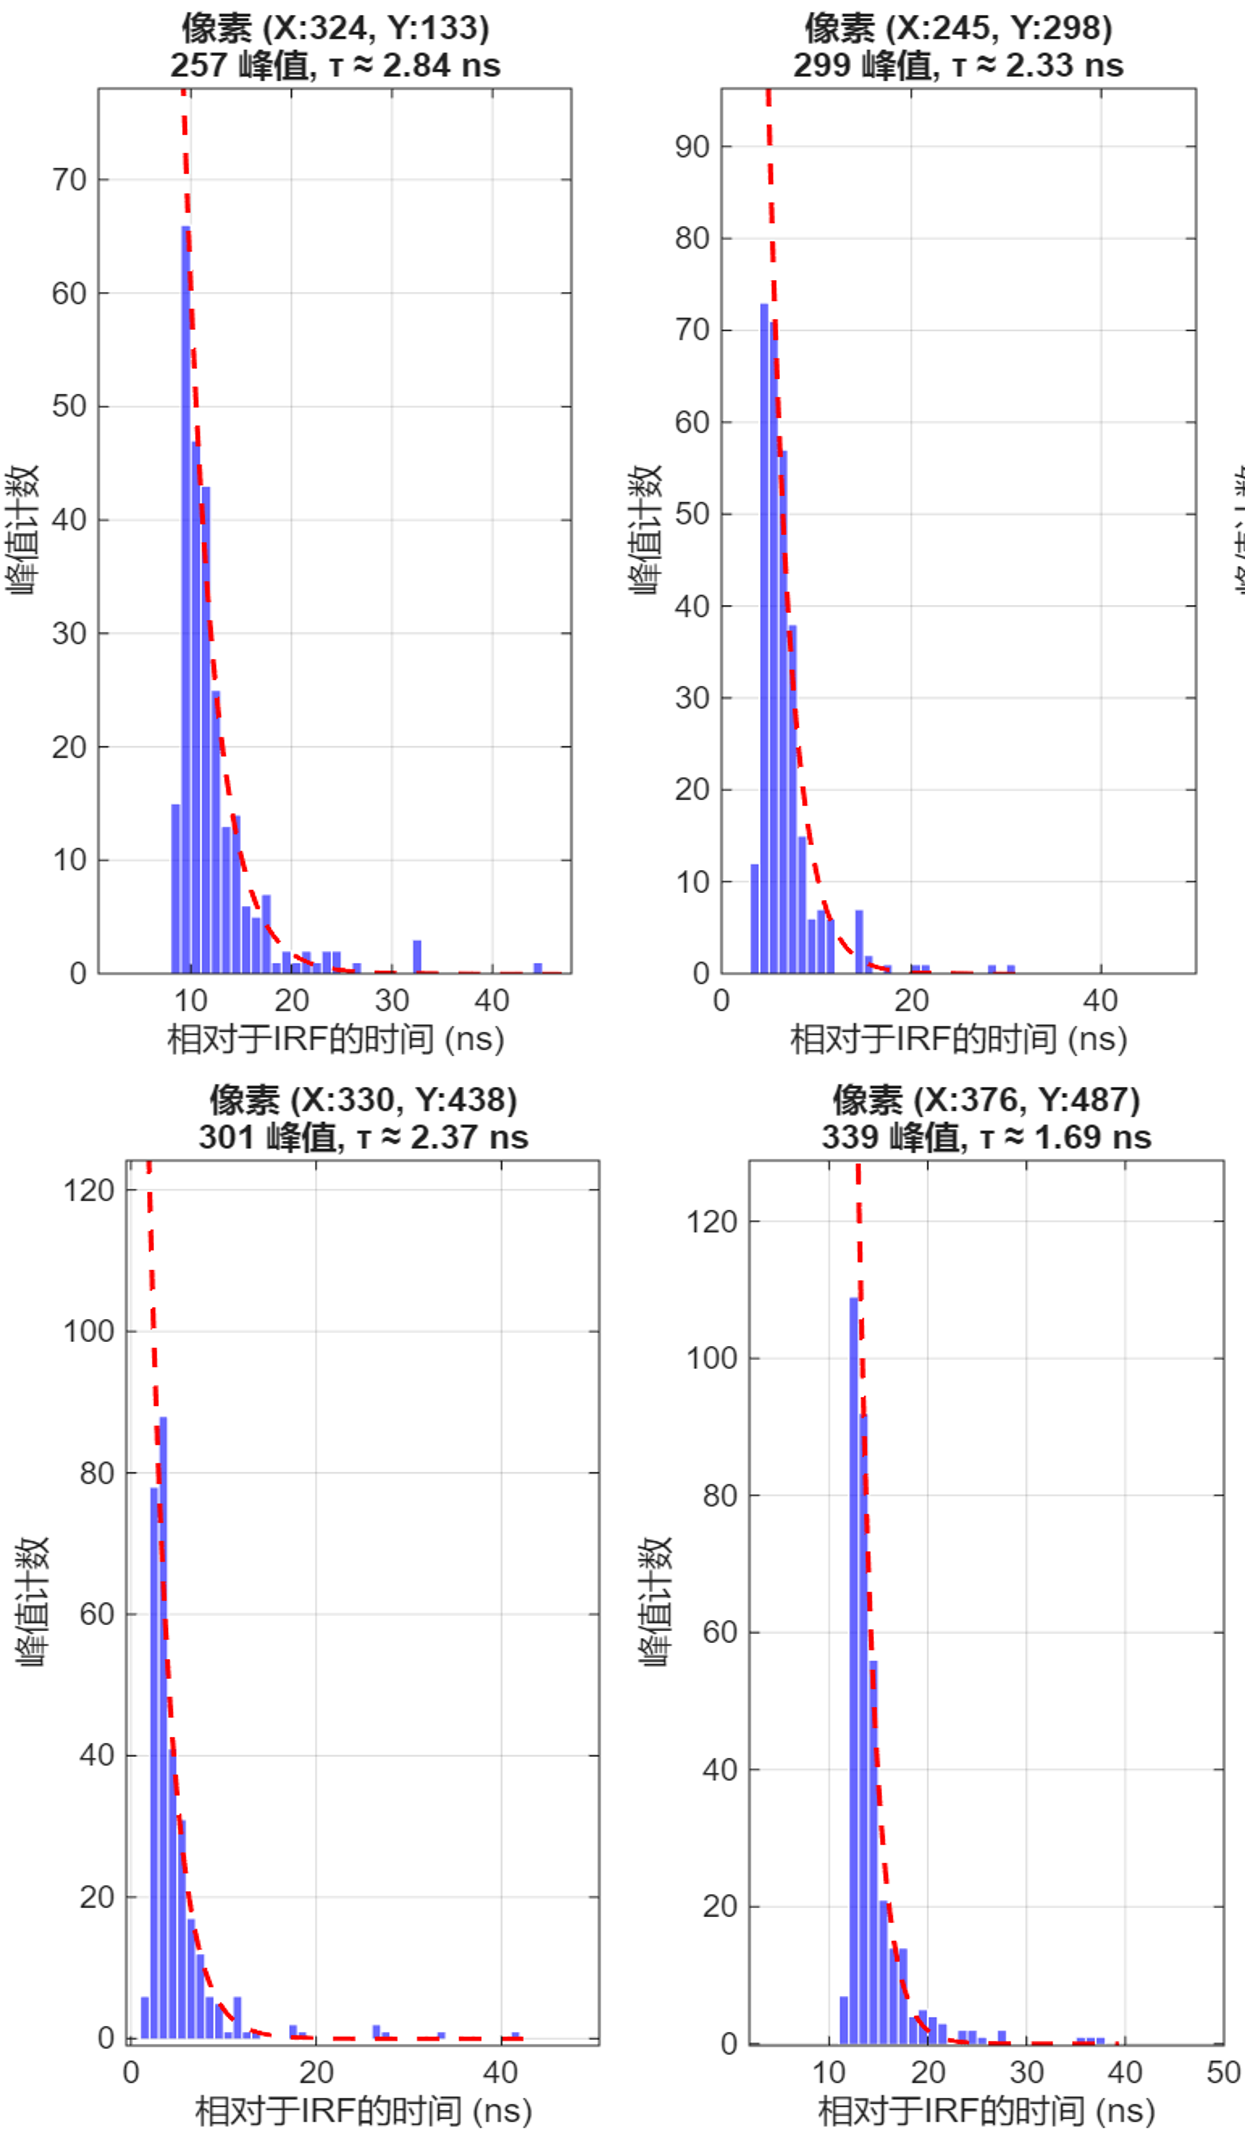
\includegraphics[width=\textwidth]{Fig/Fig28.png}
    \caption{}
    \label{fig28}
  \end{subfigure}
  \hfil
  \begin{subfigure}[b]{0.6\textwidth}
    \centering
    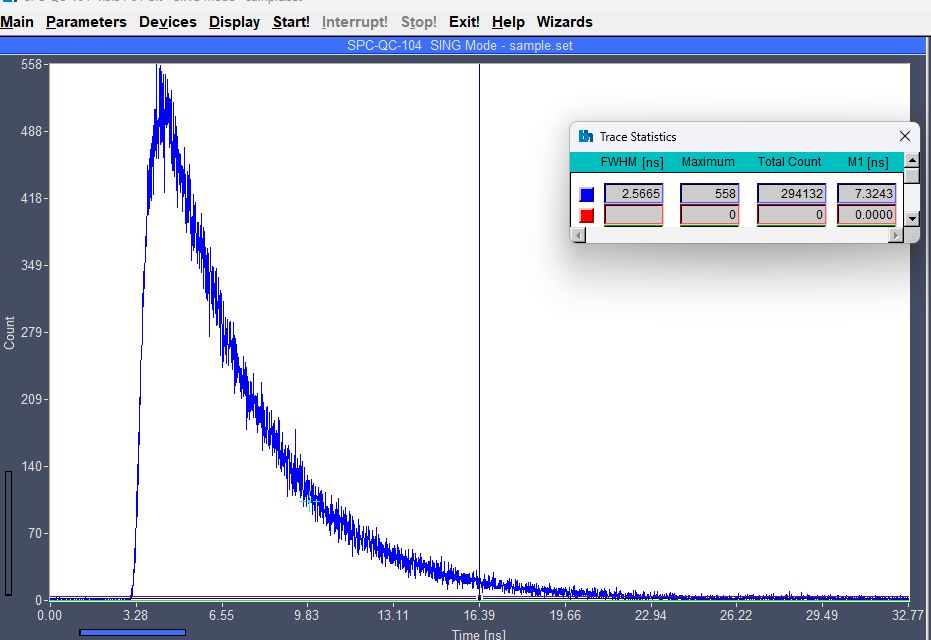
\includegraphics[width=\textwidth]{Fig/Fig28.6.png}
    \caption{}
    \label{Fig28.6}
  \end{subfigure}
  \caption{优化采集条件后的 FLIM 成像结果与逐像素寿命拟合分析。(a) 随机选取四个像素进行单指数拟合；(b) 随机选取同样样本的某个像素使用商用 SPCM 软件(Bicker \& Hickel GmbH)拟合}
  \label{fig27-28}
\end{figure}


为了进一步验证逐像素寿命拟合结果的合理性，本文在图~\ref{fig27}D 中随机选取四个像素点，对其荧光衰减曲线进行单指数拟合，结果如图~\ref{fig28} 所示。拟合得到的寿命值主要分布在 1.6--2.4\,ns 范围内，说明系统能够稳定恢复纳秒量级的寿命信息。

作为对照，图~\ref{Fig28.6} 给出了商用 SPCM 软件获得的寿命拟合结果，其代表性寿命值约为 2.4\,ns。该结果与本文自建流程得到的拟合结果处于相同量级，并在主要寿命范围上具有较好一致性。由此说明，无论是基于商用 TCSPC 板卡的三路同步成像，还是基于单路同步与逐像素重分配的自研处理流程，均能够实现对荧光寿命的有效恢复。进一步地，这也验证了本文所构建 FLIM 系统及其数据处理链路在实验上具有可行性和可靠性。


\begin{figure}[bhpt]
  \centering
  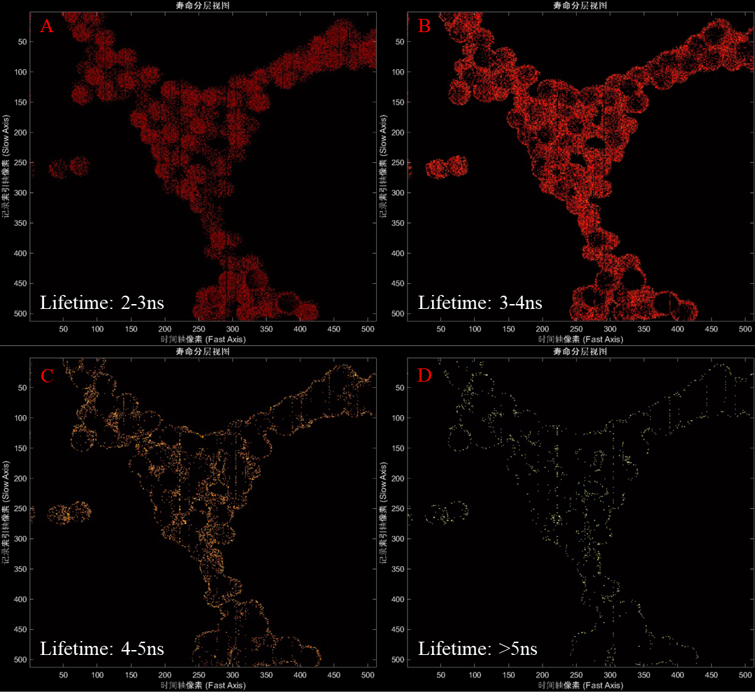
\includegraphics[width=0.6\textwidth]{Fig/Fig45.png}
  \caption{能够清晰分辨出不同荧光寿命的物质及轮廓}
  \label{fig45}
\end{figure}

图\ref{fig45}给出了在当前算法和单路同步采集模式下，利用 Acqiris 采集卡获得的荧光寿命分区结果。其中子图(A)至(D)分别对应 $2\sim3$ ns、$3\sim4$ ns、$4\sim5$ ns 和 $>5$ ns 四个寿命区间。可以看出，样品的荧光寿命主要集中在 $2\sim4$ ns 范围内，其中 $2\sim3$ ns 和 $3\sim4$ ns 区间的像素分布最为密集，结构轮廓也最为完整，说明该范围内的寿命成分占主导地位，同时当前系统在该区间内具有较高的寿命解算精度与稳定性。相比之下，$4\sim5$ ns 及 $>5$ ns 区间的像素数量较少，分布相对稀疏，表明长寿命成分所占比例较低，且对应结果更易受到噪声影响。


\section{硬件采集卡死区时间问题及优化}\label{5.6}

\begin{figure}[htbp]
  \centering
  \includegraphics[width=0.83\textwidth]{Fig/Fig29.pdf}
  \caption{SPAD 探测器与数据采集卡死区时间分析示意图}
  \label{fig29}
\end{figure}

在单光子探测系统中，系统的总死区时间不仅受限于单光子雪崩二极管(SPAD)自身的物理特性，还受到数据采集卡(DAQ)硬件响应机制的制约。图~\ref{fig29} 给出了 SPAD 探测器与数据采集卡死区时间的时序分析示意。

如图~\ref{fig29}A 所示，当 SPAD 探测到光子并产生雪崩信号后，必须经历淬灭(quenching)与恢复(recovery)过程，才能重新进入可探测下一个光子的激活状态。这一段 SPAD 无法响应新光子的时间称为 SPAD 的物理死区时间，其典型值约为 50\,ns(以 Excelitas SPCM-AQRH-14 为例)。

除前端探测器的物理死区外，后端数据采集卡的信号处理流程同样会引入硬件死区。如图~\ref{fig29}B 和图~\ref{fig29}C 所示，在标准采集窗口内，采集卡在响应一次触发信号并完成一次记录后，还需要经历数据读取和系统重置过程。经实际测量，Acqiris SA230P 采集卡的最小重置时间(rearm time)约为 23\,ns。当系统在高计数率下运行、相邻两次触发事件的间隔小于该重置时间时，采集卡将无法响应新的触发，从而导致有效光子事件丢失。


为了降低固定重置时间对系统整体探测效率的影响，本文采用了增加单次记录长度(long record)的优化策略，如图~\ref{fig29}D 所示。通过延长单次采集记录窗口，可以降低固定重置时间在总采集周期中的占比，从而提高系统的有效采集效率。系统的有效采集效率可定义为

\begin{equation}
  \eta_{\mathrm{eff}} = \frac{T_{\mathrm{record}}}{T_{\mathrm{record}} + T_{\mathrm{rearm}}}
\end{equation}

其中，$T_{\mathrm{record}}$ 为单次记录时间，$T_{\mathrm{rearm}}$ 为固定硬件重置时间。由该式可见，在 $T_{\mathrm{rearm}}$ 固定的前提下，适当增大 $T_{\mathrm{record}}$ 可以显著提高有效记录时间在整个采集周期中的占比。

然而，记录长度也不能无限增加。过长的记录窗口会使单次传输数据量显著增大，若瞬时数据流超出硬件 FIFO 缓冲能力，或整体吞吐率超过计算机内存带宽、CPU 处理速度以及 SSD 持续写入能力，就可能引发缓存溢出、数据丢失甚至系统卡顿。因此，在实际系统配置中，必须在``提高有效采集效率''和``后端数据吞吐能力''之间进行折中，以获得最合适的记录长度设置。

综上，在 FLIM 系统中，探测效率不仅取决于 SPAD 本身的性能，还受到采集卡硬件死区与后端数据处理带宽的共同限制。通过合理设置单次记录长度、优化采集参数并控制计数率，可在保证数据完整性的前提下显著提高系统的有效采集能力。


